% This LaTeX document needs to be compiled with XeLaTeX.
\documentclass[
  10
]{article}
\usepackage[margin=2cm,includehead=true,includefoot=true,centering,]{geometry}
\usepackage{xcolor}
\usepackage{ucharclasses}
\usepackage{hyperref}
\usepackage{amsmath,amssymb}
\usepackage{amsfonts}
\usepackage[version=4]{mhchem}
\usepackage{stmaryrd}
\usepackage{bbold}
\usepackage{polyglossia}
\usepackage{fontspec}
\usepackage{ctex}
\usepackage[export]{adjustbox}
\usepackage{tabularx}
\usepackage{booktabs}

\usepackage{setspace}
\setstretch{1.2}

\makeatletter
\@ifundefined{KOMAClassName}{% if non-KOMA class
  \IfFileExists{parskip.sty}{%
    \usepackage{parskip}
  }{% else
    \setlength{\parindent}{0pt}
    \setlength{\parskip}{6pt plus 2pt minus 1pt}}
}{% if KOMA class
  \KOMAoptions{parskip=half}}
\makeatother
\usepackage{longtable,booktabs,array}
\newcounter{none} % for unnumbered tables
\usepackage{multirow}
\usepackage{calc} % for calculating minipage widths
% Correct order of tables after \paragraph or \subparagraph
\usepackage{etoolbox}
\makeatletter
\patchcmd\longtable{\par}{\if@noskipsec\mbox{}\fi\par}{}{}
\makeatother
% Allow footnotes in longtable head/foot
\IfFileExists{footnotehyper.sty}{\usepackage{footnotehyper}}{\usepackage{footnote}}
\makesavenoteenv{longtable}
\usepackage{graphicx}
\makeatletter
\newsavebox\pandoc@box
\newcommand*\pandocbounded[1]{% scales image to fit in text height/width
  \sbox\pandoc@box{#1}%
  \Gscale@div\@tempa{\textheight}{\dimexpr\ht\pandoc@box+\dp\pandoc@box\relax}%
  \Gscale@div\@tempb{\linewidth}{\wd\pandoc@box}%
  \ifdim\@tempb\p@<\@tempa\p@\let\@tempa\@tempb\fi% select the smaller of both
  \ifdim\@tempa\p@<\p@\scalebox{\@tempa}{\usebox\pandoc@box}%
  \else\usebox{\pandoc@box}%
  \fi%
}
% Set default figure placement to htbp
\def\fps@figure{htbp}
\makeatother
\setlength{\emergencystretch}{3em} % prevent overfull lines
\providecommand{\tightlist}{%
  \setlength{\itemsep}{0pt}\setlength{\parskip}{0pt}}


\hypersetup{colorlinks=true, linkcolor=blue, filecolor=magenta, urlcolor=cyan,}
\urlstyle{same}

\usepackage{colortbl}
\definecolor{table-row-color}{HTML}{999999}
\definecolor{table-rule-color}{HTML}{999999}
%\arrayrulecolor{black!40}
\arrayrulecolor{table-rule-color}     % color of \toprule, \midrule, \bottomrule
\setlength{\aboverulesep}{0pt}
\setlength{\belowrulesep}{0pt}


\setotherlanguages{english}
\IfFontExistsTF{Source Han Serif CN}
{\newfontfamily\chinesefont{Source Han Serif CN}}
{\IfFontExistsTF{Noto Serif CJK SC}
  {\newfontfamily\chinesefont{Noto Serif CJK SC}}
  {\IfFontExistsTF{SimSun}
    {\newfontfamily\chinesefont{SimSun}}
    {\IfFontExistsTF{FangSong}
      {\newfontfamily\chinesefont{FangSong}}
      {\newfontfamily\chinesefont{Arial Unicode MS}}
}}}
\IfFontExistsTF{Times New Roman}
{\newfontfamily\englishfont{Times New Roman}}
{\IfFontExistsTF{Liberation Serif}
  {\newfontfamily\englishfont{Liberation Serif}}
  {\IfFontExistsTF{DejaVu Serif}
    {\newfontfamily\englishfont{DejaVu Serif}}
    {\newfontfamily\englishfont{Arial}}
}}


\author{}
\date{}

\begin{document}


\section{多功能小车}\label{ux591aux529fux80fdux5c0fux8f66}

\section{一、任务}\label{ux4e00ux4efbux52a1}

设计制作一辆小车，可沿行驶轨迹自动寻迹行驶，具备负重功能，能测量行驶轨迹中电工胶带间的宽度。

小车尺寸不大于 \(2 0 \mathrm { c m }\) （长）
\(\times 1 5 \mathrm { c m }\) （宽） \(\times 2 5 \mathrm { c m }\)
（高），小车尺寸包括小车以及所安装模块总体轮廓尺寸。小车行驶轨迹为外边长
\(1 0 0 \mathrm { c m } { \times } 1 0 0 \mathrm { c m }\)
的正方形，正方形边线为黑色，线宽
\(1 . 8 \mathrm { c m } { \pm } 0 . 2 \mathrm { c m }\)
，正方形四个顶点定义为A、B、C 和D点，示意图见图 1

\pandocbounded{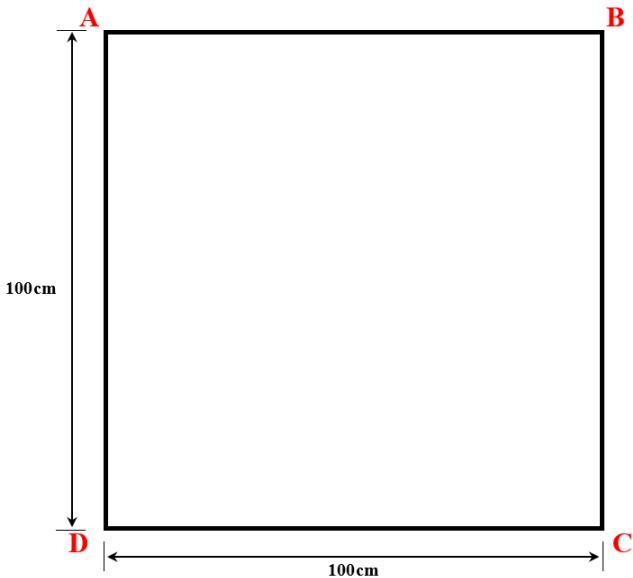
\includegraphics[keepaspectratio,alt={image}]{images/2e6221d7c91ad55e0f6847e29968a1186d918f68bda87106b92b112f5b28f7a3.jpg}}

图 1 行驶轨迹图

\section{二、要求}\label{ux4e8cux8981ux6c42}

\section{1. 基本要求}\label{ux57faux672cux8981ux6c42}

（1）将小车放置在 AB 发车点发车，小车沿行驶轨迹逆时针行驶 1
圈后停在发车点，启动和停车时需有声光提示。停车时小车前沿中心点与AD
线外沿距离 \(\mathrm { D } _ { 1 } \leq 3 ~ \mathrm { c m }\) ，行驶时间
\(t _ { 1 } \leq 1 5 \mathrm { ~ s ~ }\) 。

（2）将小车放置在AB发车点（或AD
发车点，由测评人员选择，见说明2）发车，小车可以沿布置有干扰（BC
边覆盖要求干扰 A4 纸，见说明 3）的行驶轨迹行驶 3/4 圈（AB发车点逆时针至
B 点，AD 发车点顺时针至 D
点）后掉头原路返回发车点，启动和停车时需有声光提示。停车时小车前沿中心点与终点线外沿距离
\(\mathrm { D } _ { 2 } \leq 3 ~ \mathrm { c m }\) ，行驶时间
\(t _ { 2 } \leq 2 5 \mathrm { ~ s ~ }\) 。

\section{2. 发挥部分}\label{ux53d1ux6325ux90e8ux5206}

（3）将载有 \(3 3 0 \mathrm { m l }\) 矿泉水的小车放置在AB
发车点（或AD发车点，由测评人员选择）发车，正方形CD
边的中心部位横向贴放一张待测A4纸，将待测A4纸 \(l _ { 1 }\) 和
\(l _ { 2 }\) 参数（ \(1 \ \mathrm { c m }\) \(\leq l _ { 1 }\) ,
\(l _ { 2 } { \le } 5 \mathrm { c m }\)
）通过无线传输至手机上显示，要求相对误差 \(\leq 2 0 \%\)
，小车沿行驶轨迹行驶1圈后停在发车点，启动和停车时需有声光提示。停车时小车前沿中心点与终点线外沿距离
\(\mathrm { D } _ { 3 }\) \(\leq 3 \mathrm { c m }\) ，行驶时间
\(t _ { 3 } \leq 1 5 \mathrm { ~ s ~ }\) 。

（4）将载有 \(3 3 0 \mathrm { m l }\) 矿泉水的小车放置在 AB
发车点发车，正方形 CD
边贴放一张待测A4纸，判断待测A4纸类型（圆形，正方形，三角形和椭圆形），并将小车停在行驶轨迹图对角线
AC 和 BD 三等分点对应图片位置（共 4
个点位，图形任选点位平铺放置，不重复，停车时小车外轮廓压上对应图形即可），行驶时间
\(t _ { 4 } \leq 3 0 ~ \mathrm { s }\) 。

\section{三、说明}\label{ux4e09ux8bf4ux660e}

（1）小车采用轮式小车，轮数
3\textasciitilde4个，不得采用履带和麦氏轮。小车由车载电池供电，行驶过程中不得人为干涉、遥控小车运动。``基本要求''行驶过程中小车的投影必须在轨迹线上，投影完全脱离轨迹线即认为此次测试失败，此项目不得分。进入测试环节，中途不得更换电池。

（2）发车点示意图见图 2，图 2(a)中小车前沿中心点投影在 AD
线外沿上，此位置为AB 发车点，小车按逆时针行驶，图
2(b)中小车前沿中心点投影在 AB 线外沿上，此位置为AD
发车点，小车按顺时针行驶。

\pandocbounded{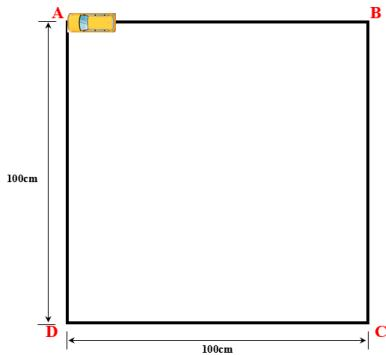
\includegraphics[keepaspectratio,alt={image}]{images/c57847e7bf8e6873121a0fc4f13807d9c2e1abffd81847c85afd6722fb46ec43.jpg}}

\begin{enumerate}
\def\labelenumi{(\alph{enumi})}
\tightlist
\item
  AB 发车点
\end{enumerate}

\pandocbounded{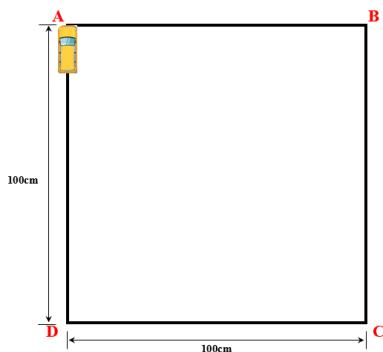
\includegraphics[keepaspectratio,alt={image}]{images/982932b37a5313ea34b2159b7d0d9751a0711e5349587a8c7abe37430d263bc2.jpg}}

\begin{enumerate}
\def\labelenumi{(\alph{enumi})}
\setcounter{enumi}{1}
\tightlist
\item
  AD 发车点
\end{enumerate}

图 2 发车点示意图

（3）干扰A4
纸，在正方形BC边的中心部位横向贴放任意一张干扰A4纸，使纵向黑色线与原 BC
行驶黑色迹线重合，该干扰 A4 纸可用 A4
纸和黑色电工胶带制作而成，共有三种类型，自备，测试时由测评人员任意选定。

（4）待测A4
纸，在正方形CD边的中心部位横向贴放任意一张待测A4纸，使纵向黑色线与原 BC
行驶黑色迹线重合，该待测 A4 纸可用 A4 纸和黑色电工胶带制作而成，共有4
种类型，进行两次测试，一次 A4待测纸自备，一次A4待测纸由测评人员提供。

\section{四、评分标准}\label{ux56dbux8bc4ux5206ux6807ux51c6}

{\def\LTcaptype{none} % do not increment counter
\begin{longtable}[]{@{}llll@{}}
\toprule\noalign{}
\endhead
\bottomrule\noalign{}
\endlastfoot
& 项 目 & 内 容 & 满 分 \\
\multirow{2}{*}{基本要求(50分)} & \multicolumn{2}{l}{%
完成第(1)项} & 20 \\
& \multicolumn{2}{l}{%
完成第(2)项} & 30 \\
\multirow{2}{*}{发挥部分(50分)} & \multicolumn{2}{l}{%
完成第(1)项} & 30 \\
& \multicolumn{2}{l}{%
完成第(2)项} & 20 \\
\multirow{5}{*}{设计报告(20分)} & 系统方案 & 方案比较与选择 &
\multirow{5}{*}{20} \\
& 理论分析与计算 & 数字识别、自动寻径方法 \\
& 程序设计 & 流程图 \\
& 测试方案和结果 & 测试方案结果和分析 \\
& 报告结构及规范性 & 摘要,正文结构,图表规范性 \\
\multicolumn{3}{@{}l}{%
总 分} & 120 \\
\end{longtable}
}

\end{document}
